\documentclass[12pt,ignorenonframetext,compress]{beamer}
\setbeamertemplate{caption}[numbered]
\setbeamertemplate{caption label separator}{: }
\setbeamercolor{caption name}{fg=normal text.fg}
\beamertemplatenavigationsymbolsempty
\usepackage{lmodern}
\usepackage{amssymb,amsmath}
\usepackage{ifxetex,ifluatex}
\usepackage{fixltx2e} % provides \textsubscript
\ifnum 0\ifxetex 1\fi\ifluatex 1\fi=0 % if pdftex
\usepackage[T1]{fontenc}
\usepackage[utf8]{inputenc}
\else % if luatex or xelatex
\ifxetex
\usepackage{mathspec}
\else
\usepackage{fontspec}
\fi
\defaultfontfeatures{Ligatures=TeX,Scale=MatchLowercase}
\fi
\usetheme{metropolis}
% use upquote if available, for straight quotes in verbatim environments
\IfFileExists{upquote.sty}{\usepackage{upquote}}{}
% use microtype if available
\IfFileExists{microtype.sty}{%
\usepackage{microtype}
\UseMicrotypeSet[protrusion]{basicmath} % disable protrusion for tt fonts
}{}
\newif\ifbibliography
\usepackage{graphicx,grffile}
\makeatletter
\def\maxwidth{\ifdim\Gin@nat@width>\linewidth\linewidth\else\Gin@nat@width\fi}
\def\maxheight{\ifdim\Gin@nat@height>\textheight0.8\textheight\else\Gin@nat@height\fi}
\makeatother
% Scale images if necessary, so that they will not overflow the page
% margins by default, and it is still possible to overwrite the defaults
% using explicit options in \includegraphics[width, height, ...]{}
\setkeys{Gin}{width=\maxwidth,height=\maxheight,keepaspectratio}

% Prevent slide breaks in the middle of a paragraph:
\widowpenalties 1 10000
\raggedbottom

\AtBeginPart{
\let\insertpartnumber\relax
\let\partname\relax
\frame{\partpage}
}
\AtBeginSection{
\ifbibliography
\else
\let\insertsectionnumber\relax
\let\sectionname\relax
\frame{\sectionpage}
\fi
}
\AtBeginSubsection{
\let\insertsubsectionnumber\relax
\let\subsectionname\relax
\frame{\subsectionpage}
}

\setlength{\parindent}{0pt}
\setlength{\parskip}{6pt plus 2pt minus 1pt}
\setlength{\emergencystretch}{3em}  % prevent overfull lines
\providecommand{\tightlist}{%
\setlength{\itemsep}{0pt}\setlength{\parskip}{0pt}}
\setcounter{secnumdepth}{0}
%% header.tex
%%
%% Copyright (C) 2016 - 2017  Dirk Eddelbuettel
%%
%% This file is part of samples-rmarkdown-metropolis repository.
%%
%% samples-rmarkdown-metropolis is free software: you can redistribute it
%% and/or modify it under the terms of the GNU General Public License as
%% published by the Free Software Foundation, either version 2 of the
%% License, or (at your option) any later version.
%%
%% samples-rmarkdown-metropolis is distributed in the hope that it will be
%% useful, but WITHOUT ANY WARRANTY; without even the implied warranty of
%% MERCHANTABILITY or FITNESS FOR A PARTICULAR PURPOSE.  See the GNU General
%% Public License for more details.
%%
%% You should have received a copy of the GNU General Public License along with
%% samples-rmarkdown-metropolis.  If not, see <http://www.gnu.org/licenses/>.

%% If you have the Fira font installed, to actually have it used it 
%% via rmarkdown you need to declare it here 
%\setsansfont[ItalicFont={Fira Sans Light Italic},BoldFont={Fira Sans},BoldItalicFont={Fira Sans Italic}]{Fira Sans Light}
%\setmonofont[BoldFont={Fira Mono Medium}]{Fira Mono}
%\usepackage[orientation=landscape,size=custom,width=16,height=9,scale=0.5,debug]{beamerposter}
\setbeamertemplate{footline}[frame number]
%% You can set various Metropolis options via \metroset{} here
%\metroset{....}
%% You can redefine colours, mostly by borrowing from Beamer
\setbeamercolor{frametitle}{bg=gray}

%% You also use hyperref, and pick colors 
\hypersetup{colorlinks,citecolor=orange,filecolor=red,linkcolor=brown,urlcolor=blue}

%% when rendered with rmarkdown, somehow the unicode char for the dot
%% disappears so we redefine it here -- that is an older comments, seems font-specific
%\renewcommand{\textbullet}{$\cdot$}
%\renewcommand{\itemBullet}{▸}   % unicode U+25b8 'black right pointing small triangle'

%% The institute macro puts a small line for affiliation at the bottom
\institute{Beihang University} 

%% We can also place a logo
%%\titlegraphic{\hfill
\includegraphics[height=1cm]{figures/buaalogo.jpg}}

%%% Local Variables:
%%% mode: latex
%%% TeX-master: t
%%% End:

\title{Forecasting performance evaluation in time series instance spaces}
\subtitle{Talk at BUAA}
\author{Yanfei Kang, Rob Hyndman and Kate Smith-Miles}
\date{Oct 25, 2017}

\begin{document}
\frame{\titlepage}

\section{Motivation}\label{motivation}

\begin{frame}{M3 data}

\centerline{
\includegraphics[width=\textwidth]{figures/M3paper.png}}

\end{frame}

\begin{frame}{M3 data}

\begin{itemize}
\tightlist
\item
  3003 time series
\item
  From demography, finance, business and economics
\item
  Lengths between 14 and 126
\item
  Either non-seasonal, monthly or quarterly
\item
  Positive
\end{itemize}

\end{frame}

\begin{frame}{Questions}

\begin{itemize}
\item
  Do we favour forecasting methods that work well with specific types of
  data?
\item
  How diverse and challenging are these time series?
\item
  Are there particular features of some time series that make them
  particularly amenable to being forecast by one method compared to
  another?
\end{itemize}

\end{frame}

\begin{frame}{What we do}

\begin{itemize}
\tightlist
\item
  Visualize M3 data in feature space.
\item
  Study the distribution of their features.
\item
  Identify gaps in the instance space, and generate new time series with
  controllable features given a target location.
\item
  Predict forecasting method performance in the instance space.
\end{itemize}

\end{frame}

\section{Time series features}\label{time-series-features}

\begin{frame}{Basic idea}

Transform a given time series \(\{x_1, x_2, \cdots, x_n\}\) to a feature
vector \(F = (F_1, F_2, \cdots, F_p)'\).

\begin{block}{Why?}

\begin{enumerate}
\def\labelenumi{\arabic{enumi}.}
\tightlist
\item
  When the time series is very long, this is kind of dimension
  reduction.
\item
  It deals with time series with different lengths.
\item
  Focus on shapes.
\end{enumerate}

\end{block}

\end{frame}

\begin{frame}{Time series features}

\metroset{block=fill}

\begin{alertblock}{The six features used to characterize a time series.}
\begin{enumerate}
\item Spectral entropy
\item Strength of trend
\item Strength of seasonality
\item Seasonal period
\item First order autocorrelation
\item Optimal Box-Cox transformation parameter
\end{enumerate} 
\end{alertblock}

\end{frame}

\begin{frame}{Spectral entropy \(F_1\)}

We use an estimate of the Shannon entropy of the spectral density
\(f_x(\lambda)\) of a stationary process \(x_t\): \[
    F_1 = - \int_{-\pi}^{\pi} \hat{f}_x(\lambda) \log \hat{f}_x(\lambda) d\lambda,
\] where \(\hat{f}_x(\lambda)\) is an estimate of the spectrum of the
time series.

\begin{itemize}
\tightlist
\item
  Small \(F_1\) \(\Rightarrow\) more signal and more forecastable.
\item
  Relative larger \(F_1\) \(\Rightarrow\) more uncertainty and harder to
  forecast.
\end{itemize}

\end{frame}

\begin{frame}{Strength of trend \(F_2\) and strength of seasonality
\(F_3\)}

\begin{block}{STL decompostion}

\[ x_t = S_t + T_t + R_t.\] The strength of trend can be measured by
comparing the variances of \(R_t\) and \(x_t - S_t\). \[
    F_2 = 1- \frac{\text{var}(R_t)}{\text{var}(x_t - S_t)}.
\]

The strength of seasonality is defined as:

\[
F_3 = 1- \frac{\text{var}(R_t)}{\text{var}(x_t - T_t)}.
\]

\end{block}

\end{frame}

\begin{frame}[fragile]{Seasonal period \(F_4\)}

\begin{itemize}
\tightlist
\item
  \(F_4=12\) for monthly data
\item
  \(F_4=4\) for quarterly data
\item
  \(F_4=1\) for nonseasonal data
\item
  When the period is unknown, it could be estimated from the data using,
  for example, the \texttt{findfrequency()} function from the
  \textbf{forecast} package in \textbf{R}.
\end{itemize}

\end{frame}

\begin{frame}{First order autocorrelation \(F_5\)}

ACF is greatly affected by trend and seasonality, so we compute the
autocorrelations in \(\{R_t\}\): \[
F_5 = \text{Corr}(R_t,R_{t-1}).
\]

\end{frame}

\begin{frame}{Optimal Box-Cox transformation parameter \(F_6\)}

\begin{block}{Box-Cox transformation}

\[
\begin{aligned}
& \\
&    w_t=
    \begin{cases}
      \log(x_t),               & \text{if }\lambda = 0, \\
      (x_t^\lambda-1)/\lambda, & \text{otherwise}.
    \end{cases}
\end{aligned}
\]

\begin{itemize}
\item
  A good \(\lambda\) makes the variation of a series approximately
  constant across the whole series.
\item
  We choose \(\lambda \in (0, 1)\) to maximise the profile log
  likelihood of a linear model fitted to \(x_t\).
\item
  Measures the degree of change of variation in the data.
\end{itemize}

\end{block}

\end{frame}

\begin{frame}{M3 time series features}

\centerline{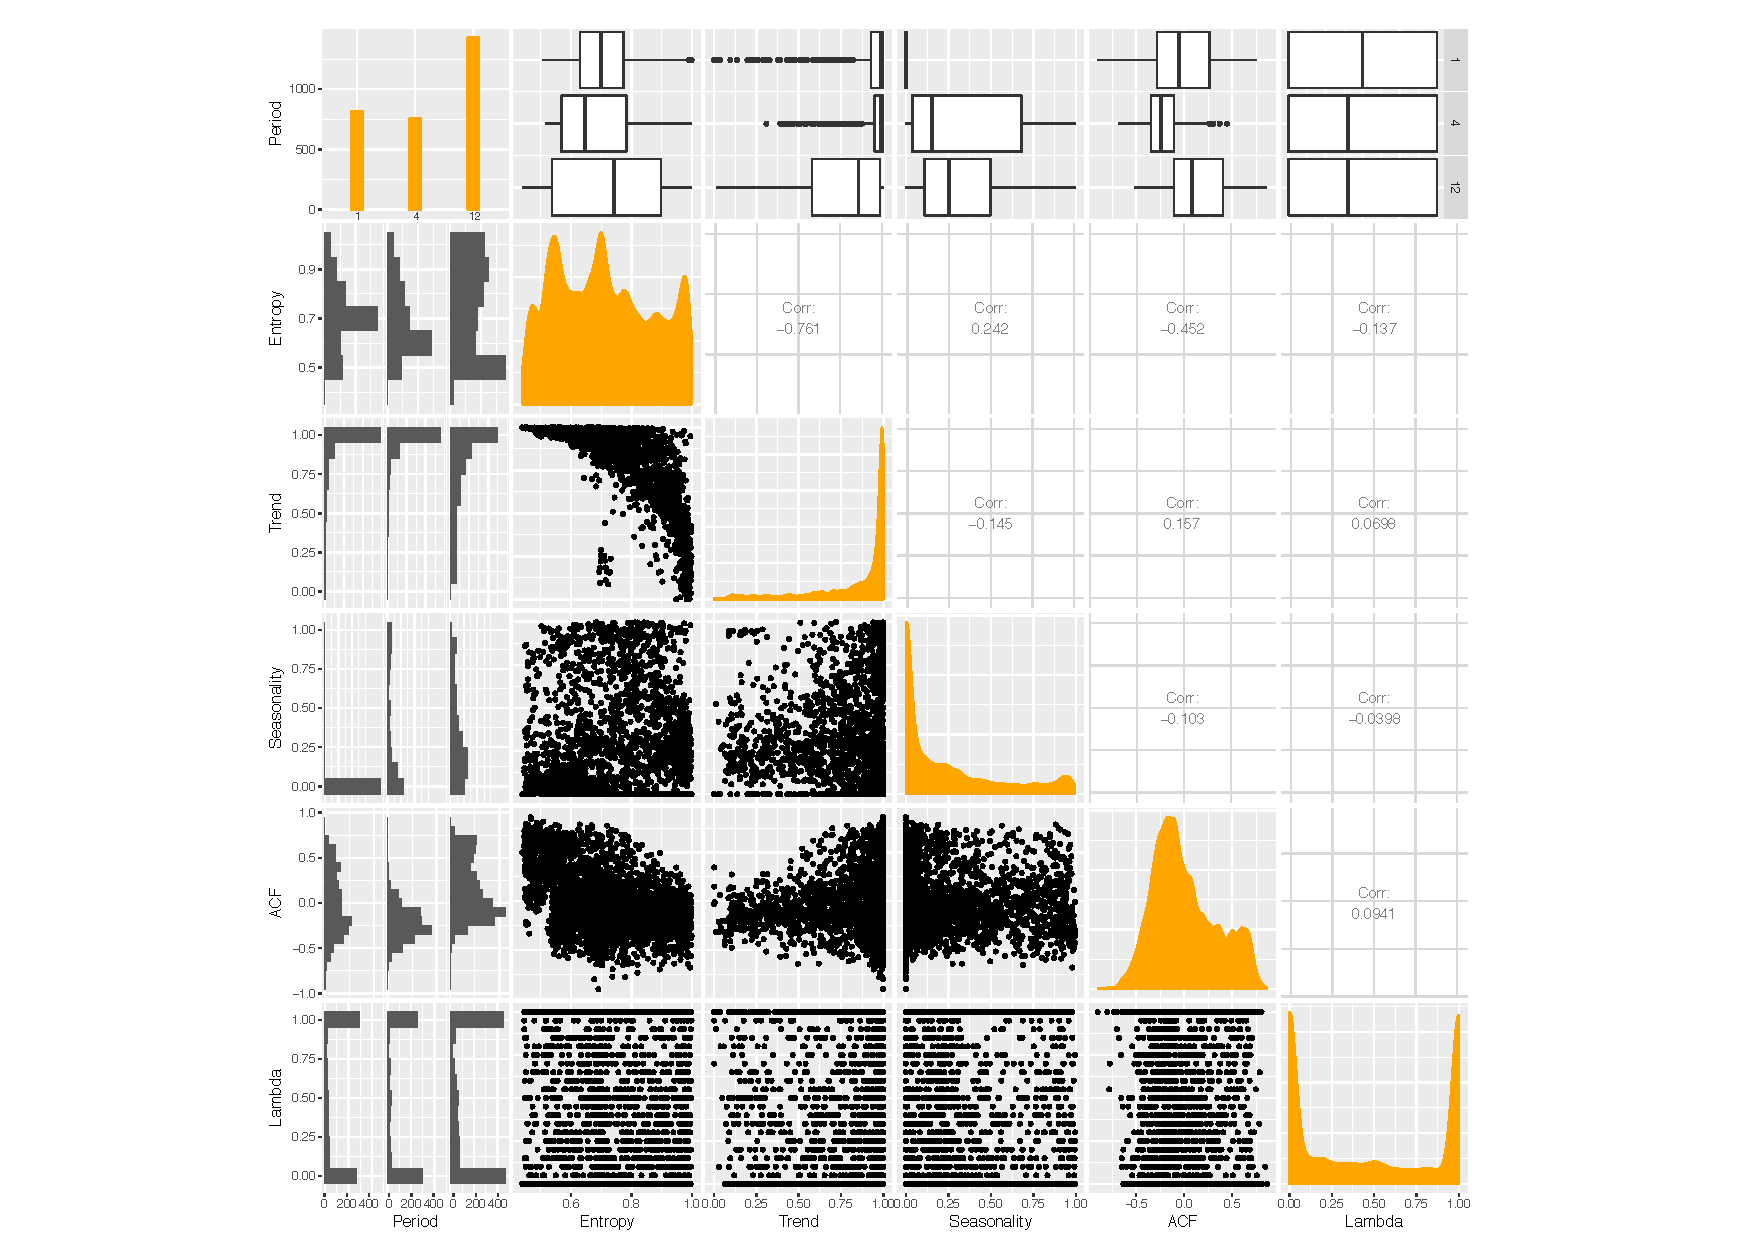
\includegraphics[width=\textwidth]{figures/PairwisePlot.pdf}}

\end{frame}

\begin{frame}{Visualisation}

\begin{itemize}
\tightlist
\item
  PCA
\end{itemize}

\[
  \begin{bmatrix}
    \text{PC1} \\
    \text{PC2}
  \end{bmatrix}
  =
  \begin{bmatrix}
    0.614 & -0.588 &  0.321 &  0.258 & -0.292 & -0.150  \\
    0.210 & 0.000 &  -0.307 &  -0.687 & -0.608 &  -0.114
  \end{bmatrix}\textbf{F}
\]

\begin{itemize}
\item
  PC1 increases with spectral entropy and decreases with trend and first
  order autocorrelation.
\item
  PC2 negatively depicts period and seasonality.
\end{itemize}

\end{frame}

\begin{frame}{Feature space of M3}

\centerline{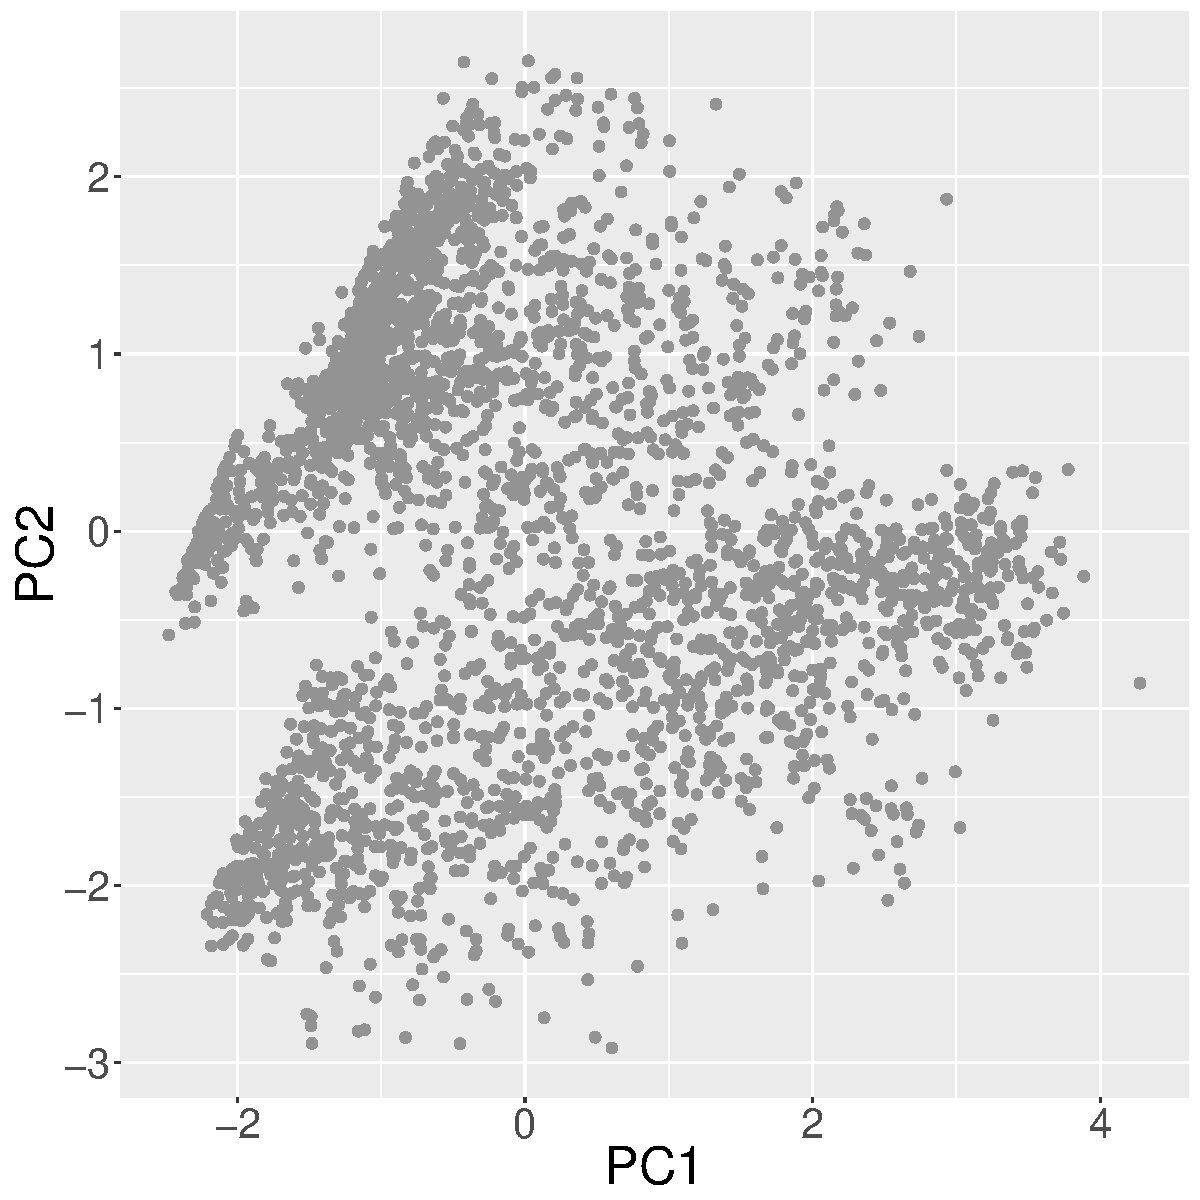
\includegraphics[width=\textwidth]{figures/InstanceSpace0.pdf}}

\end{frame}

\begin{frame}{Feature distributions of M3}

\centerline{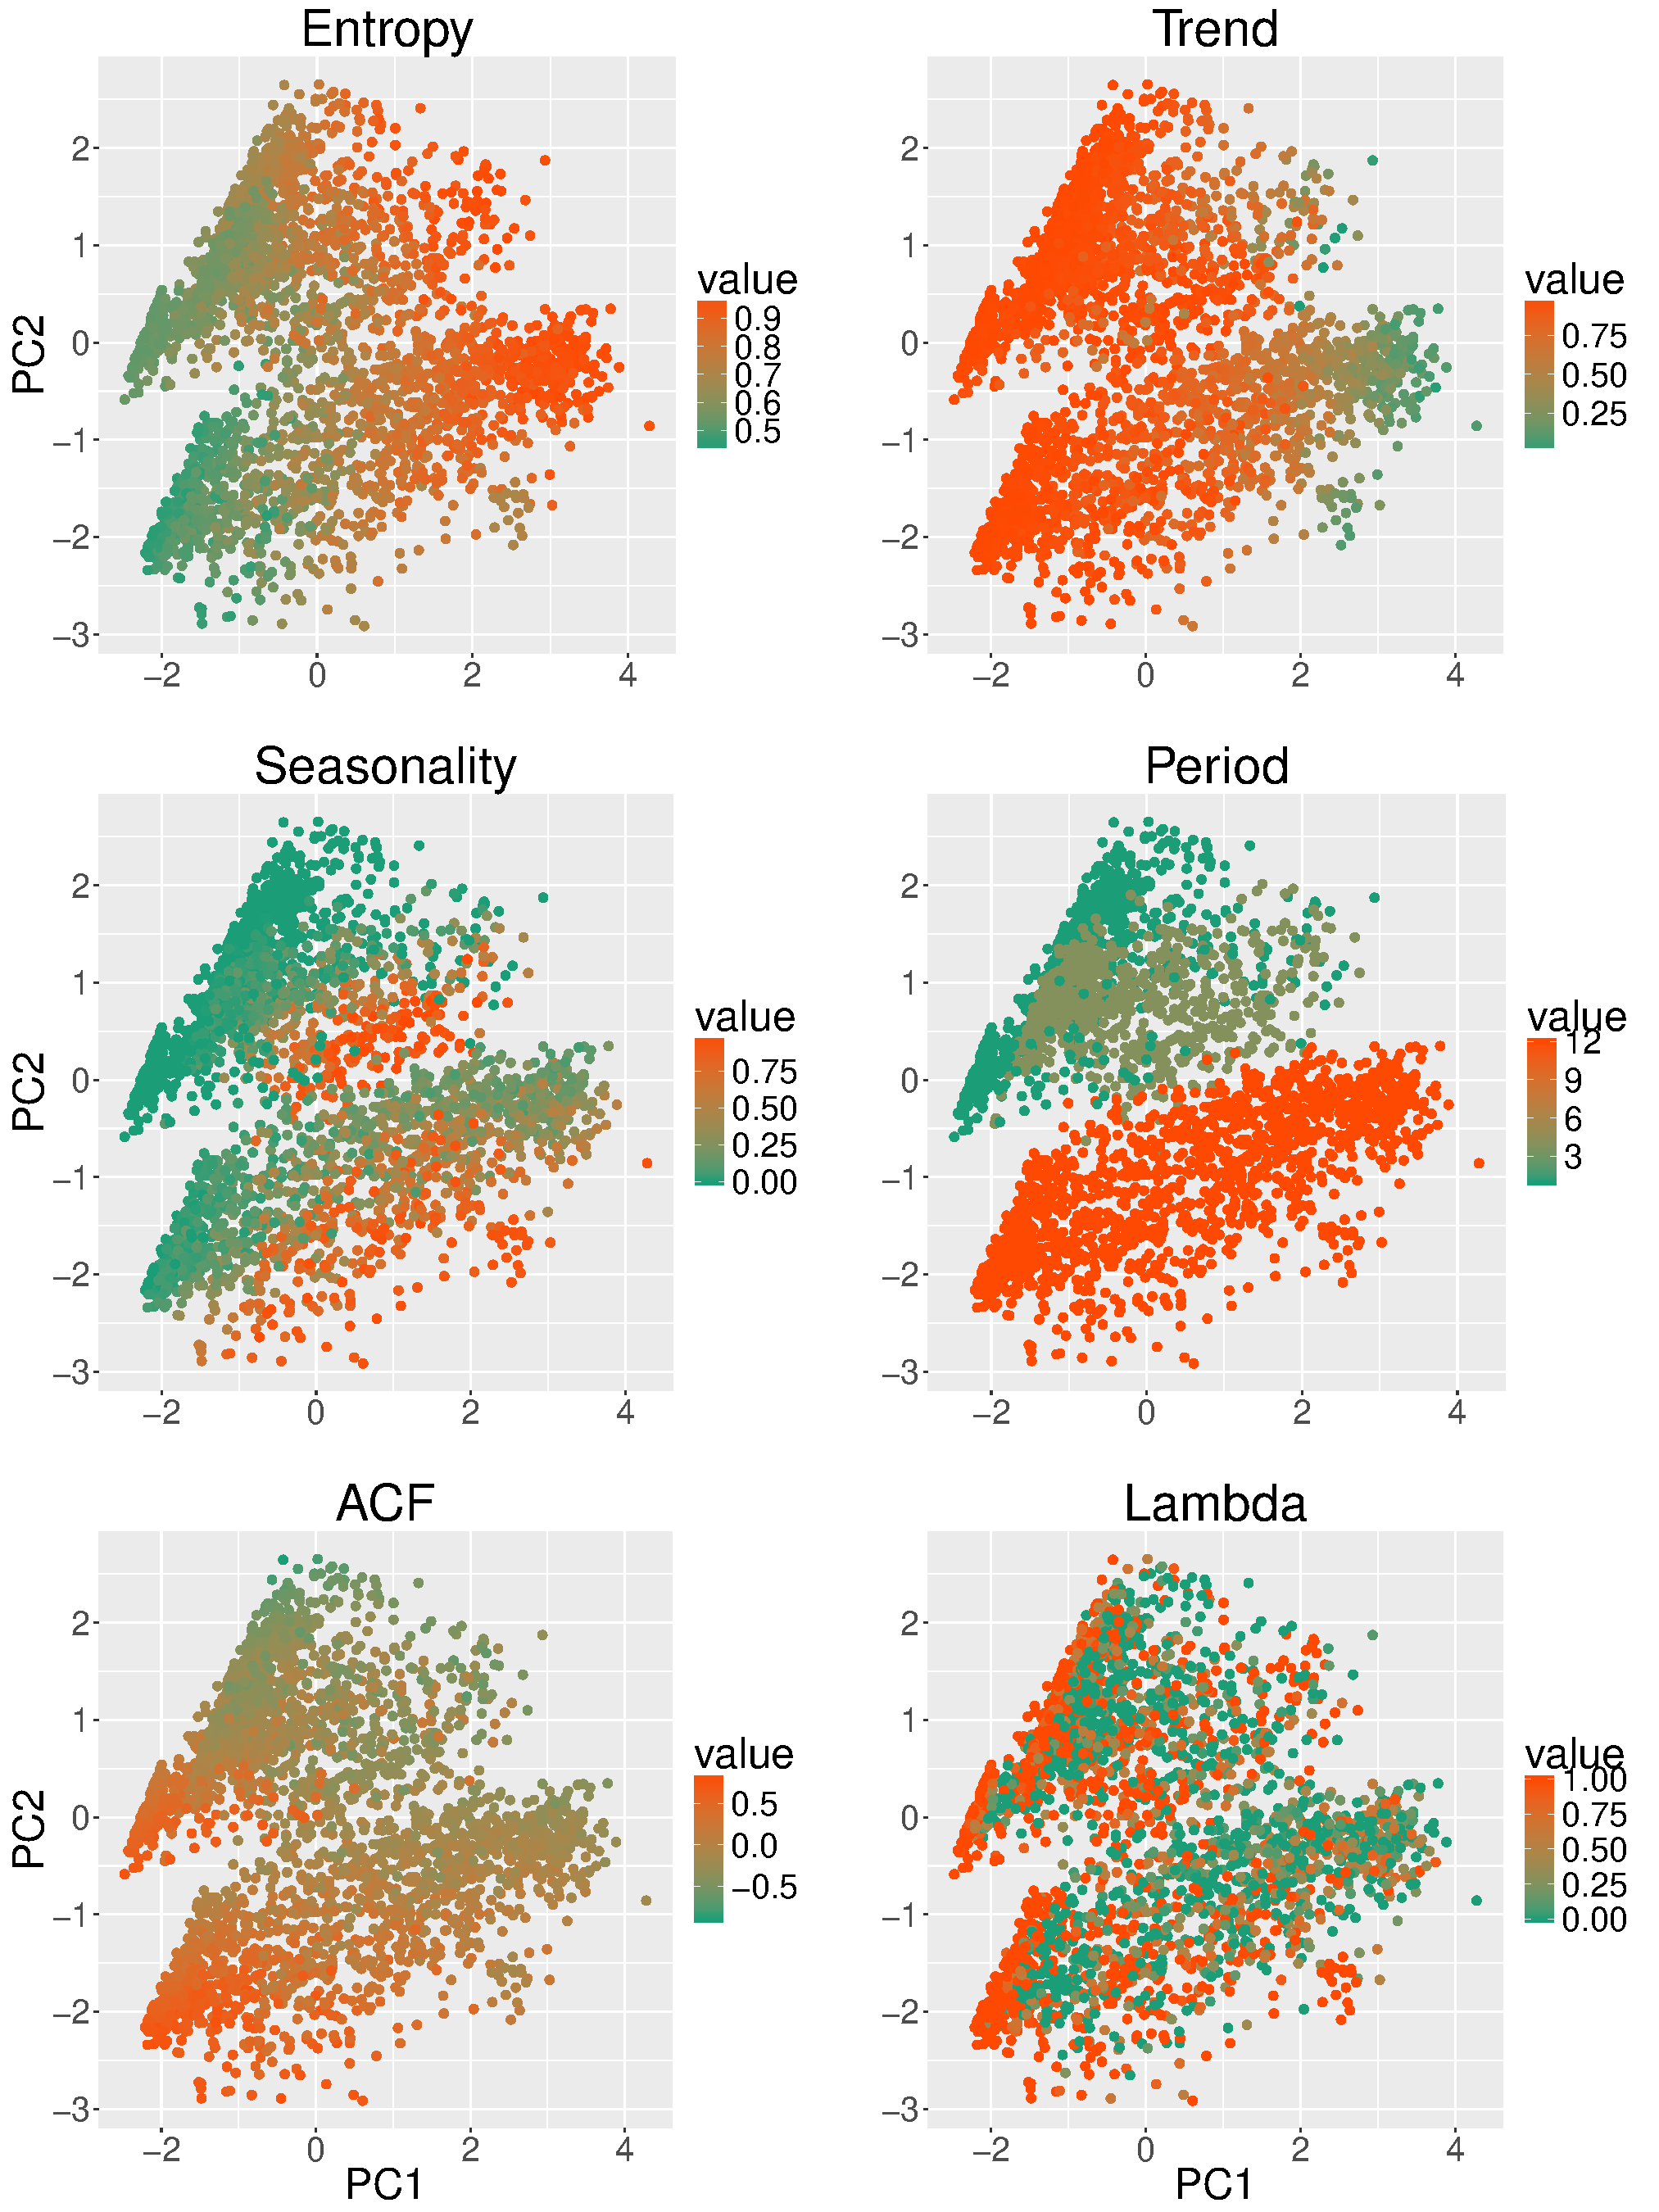
\includegraphics[width=\textwidth]{figures/FeatureDistribution.pdf}}

\end{frame}

\begin{frame}{Questions}

\begin{columns}[T]
    \begin{column}{.5\textwidth}
    \begin{block}{}
    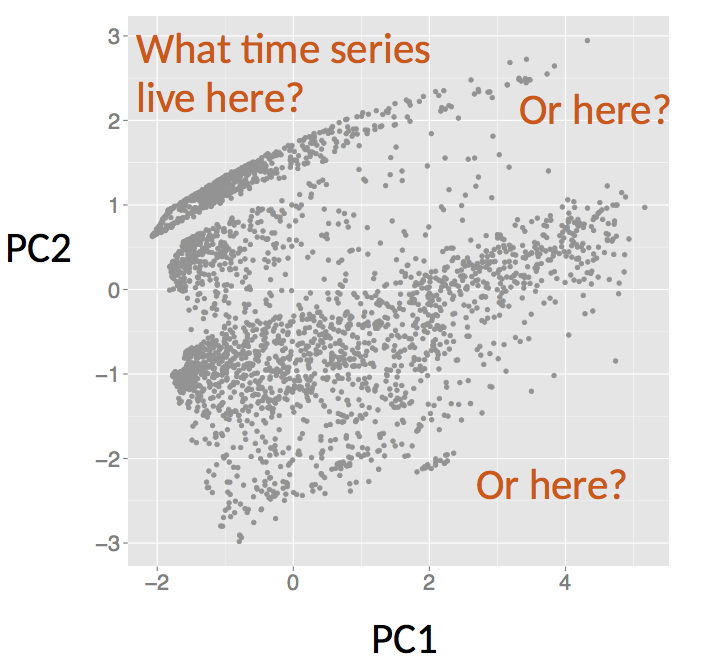
\includegraphics[width=\textwidth]{figures/holes.png}
    \end{block}
    \end{column}
     \begin{column}{.5\textwidth}
     \begin{block}{}
        \begin{itemize}
          \item Is it possible to fill and extend the whole space? or
          \item Can we generate a more diverse set of time series than M3?
        \end{itemize}
    \end{block}
    \end{column}
  \end{columns}

\end{frame}

\section{New time series generation in feature
space}\label{new-time-series-generation-in-feature-space}

\begin{frame}{New time series generation}

\begin{itemize}
\item
  Once a target point is set, our goal is to evolve a new time series
  instance which is as close as possible to the target point.
\item
  The process relies on a genetic algorithm (GA). Initial populations
  are improved until the final population is achieved with maximised
  fitness.
\end{itemize}

\end{frame}

\begin{frame}{GA procedure}

For each target point \(T_i\), \(i = 1, 2, \dots, N_t\), we first
generate an initial population of time series and iterate until the
whole process meets some convergence criteria:

\begin{enumerate}
\def\labelenumi{\arabic{enumi}.}
\tightlist
\item
  Calculate the feature vector for each time series
  \(j \in \{1, 2, \dots, N_p\}\) in the current population. Project it
  into 2-d: \(\text{PC}_j\).
\item
  Calculate the fitness of each member in the current population: \[
        \text{Fitness}(j) = - \sqrt{(|\text{PC}_j-T_i|^2)}.
      \]
\item
  Evolve the next generation based on the fittest individuals.
\end{enumerate}

From the final population, we select the instance closest to the target
point.

\end{frame}

\begin{frame}{Validation}

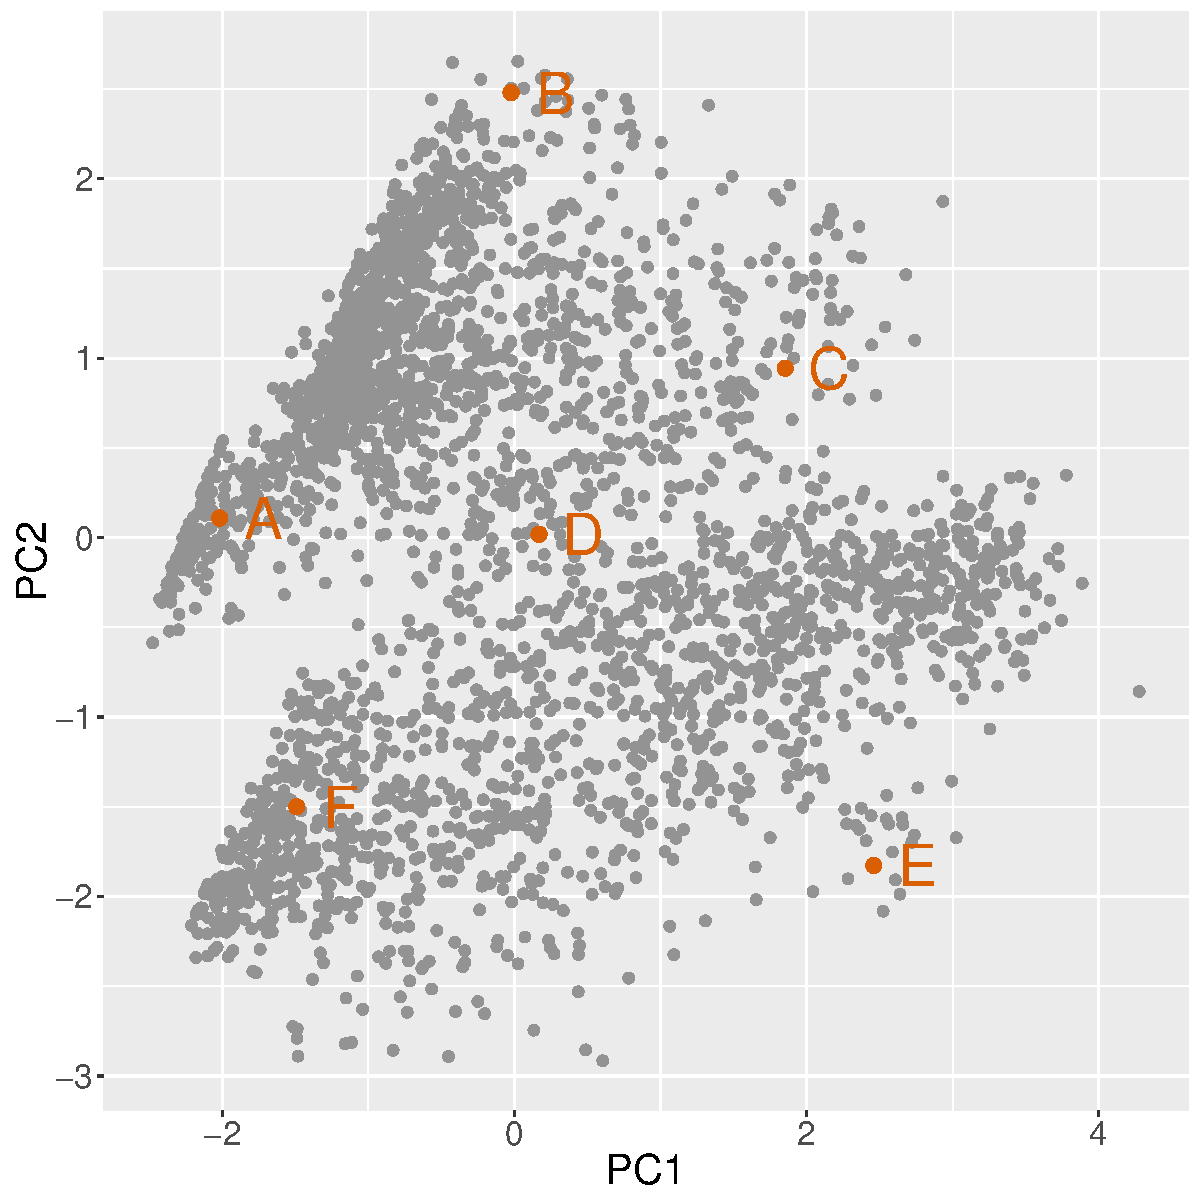
\includegraphics[width=0.4\textwidth]{figures/TargetedInstancesEgsLocations.pdf}
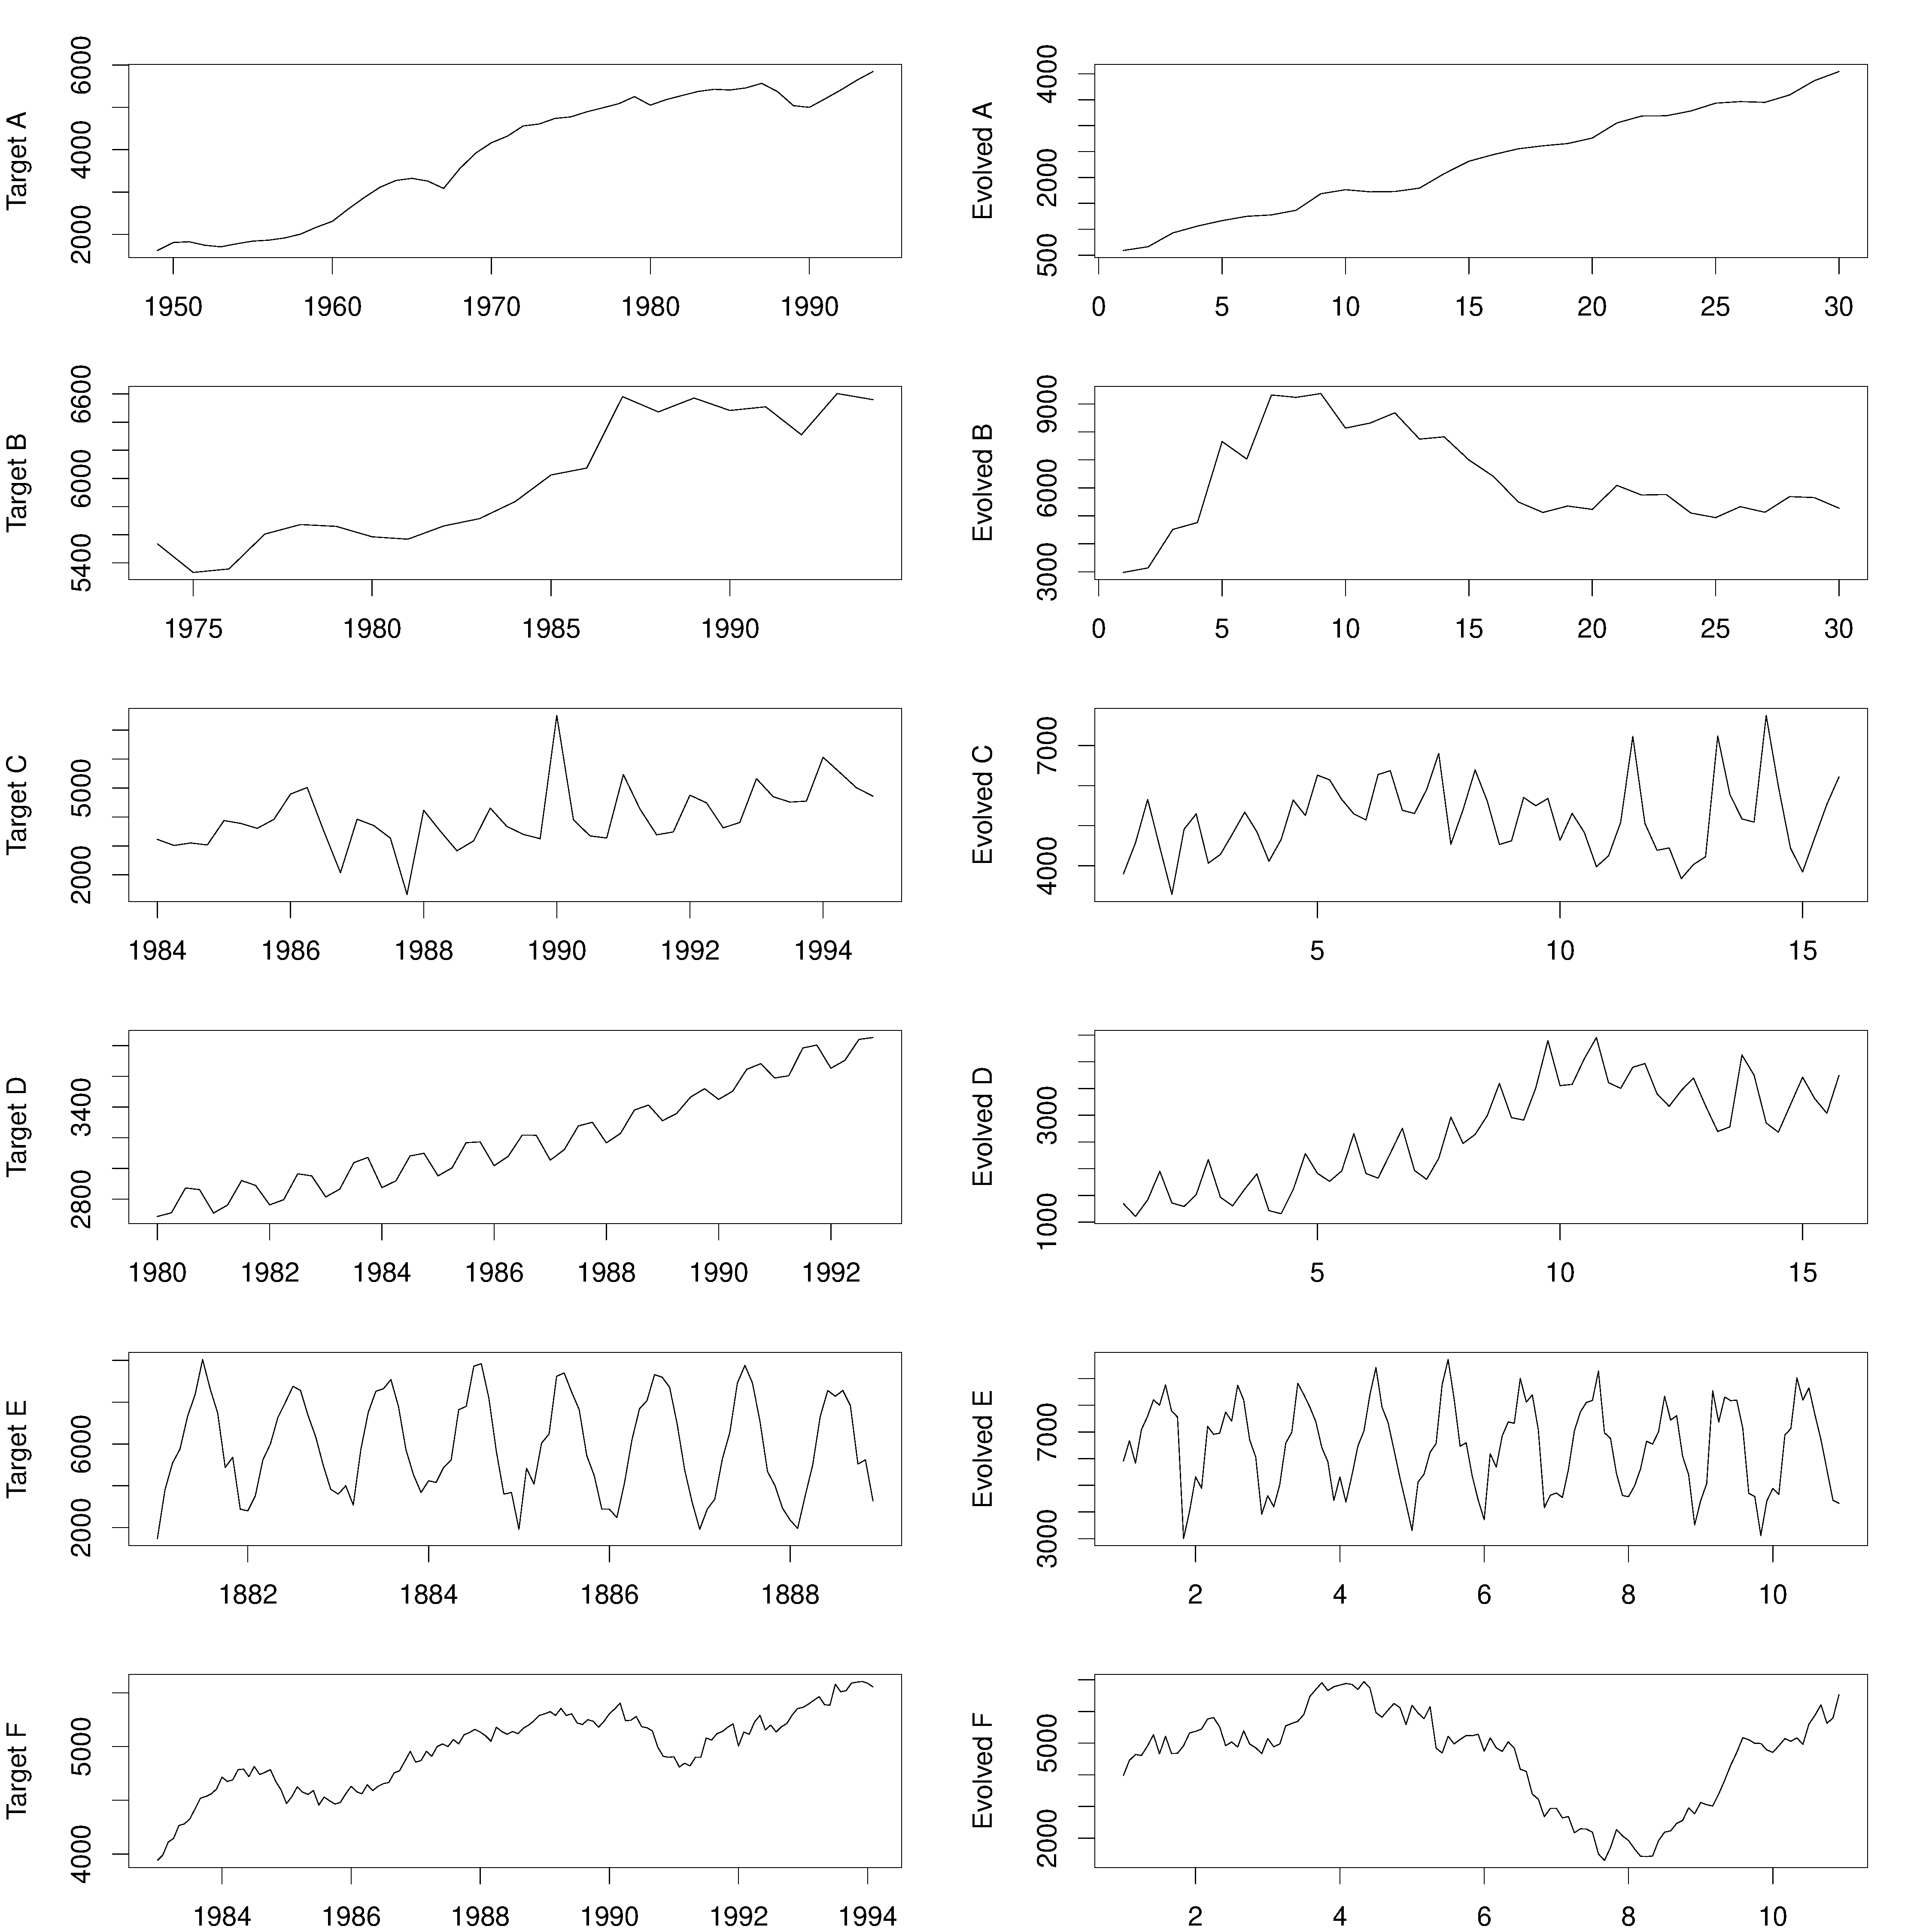
\includegraphics[width=0.7\textwidth]{figures/EvolvedInstancesEgs.pdf}

\end{frame}

\begin{frame}{Validation}

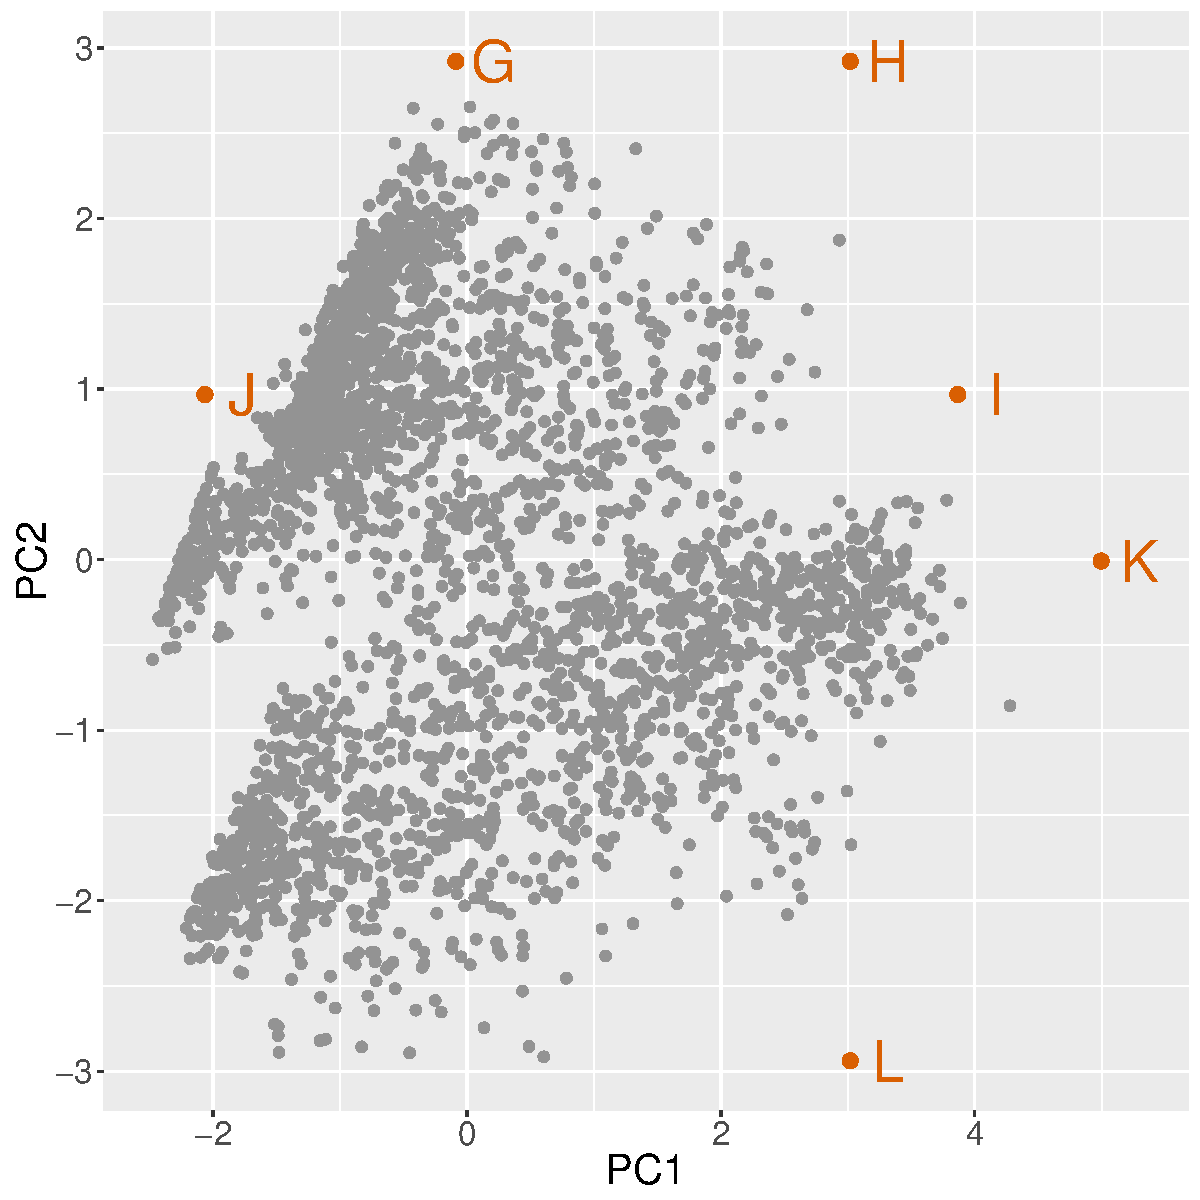
\includegraphics[width=0.4\textwidth]{figures/UnknownEvolvedEgsLocations.pdf}
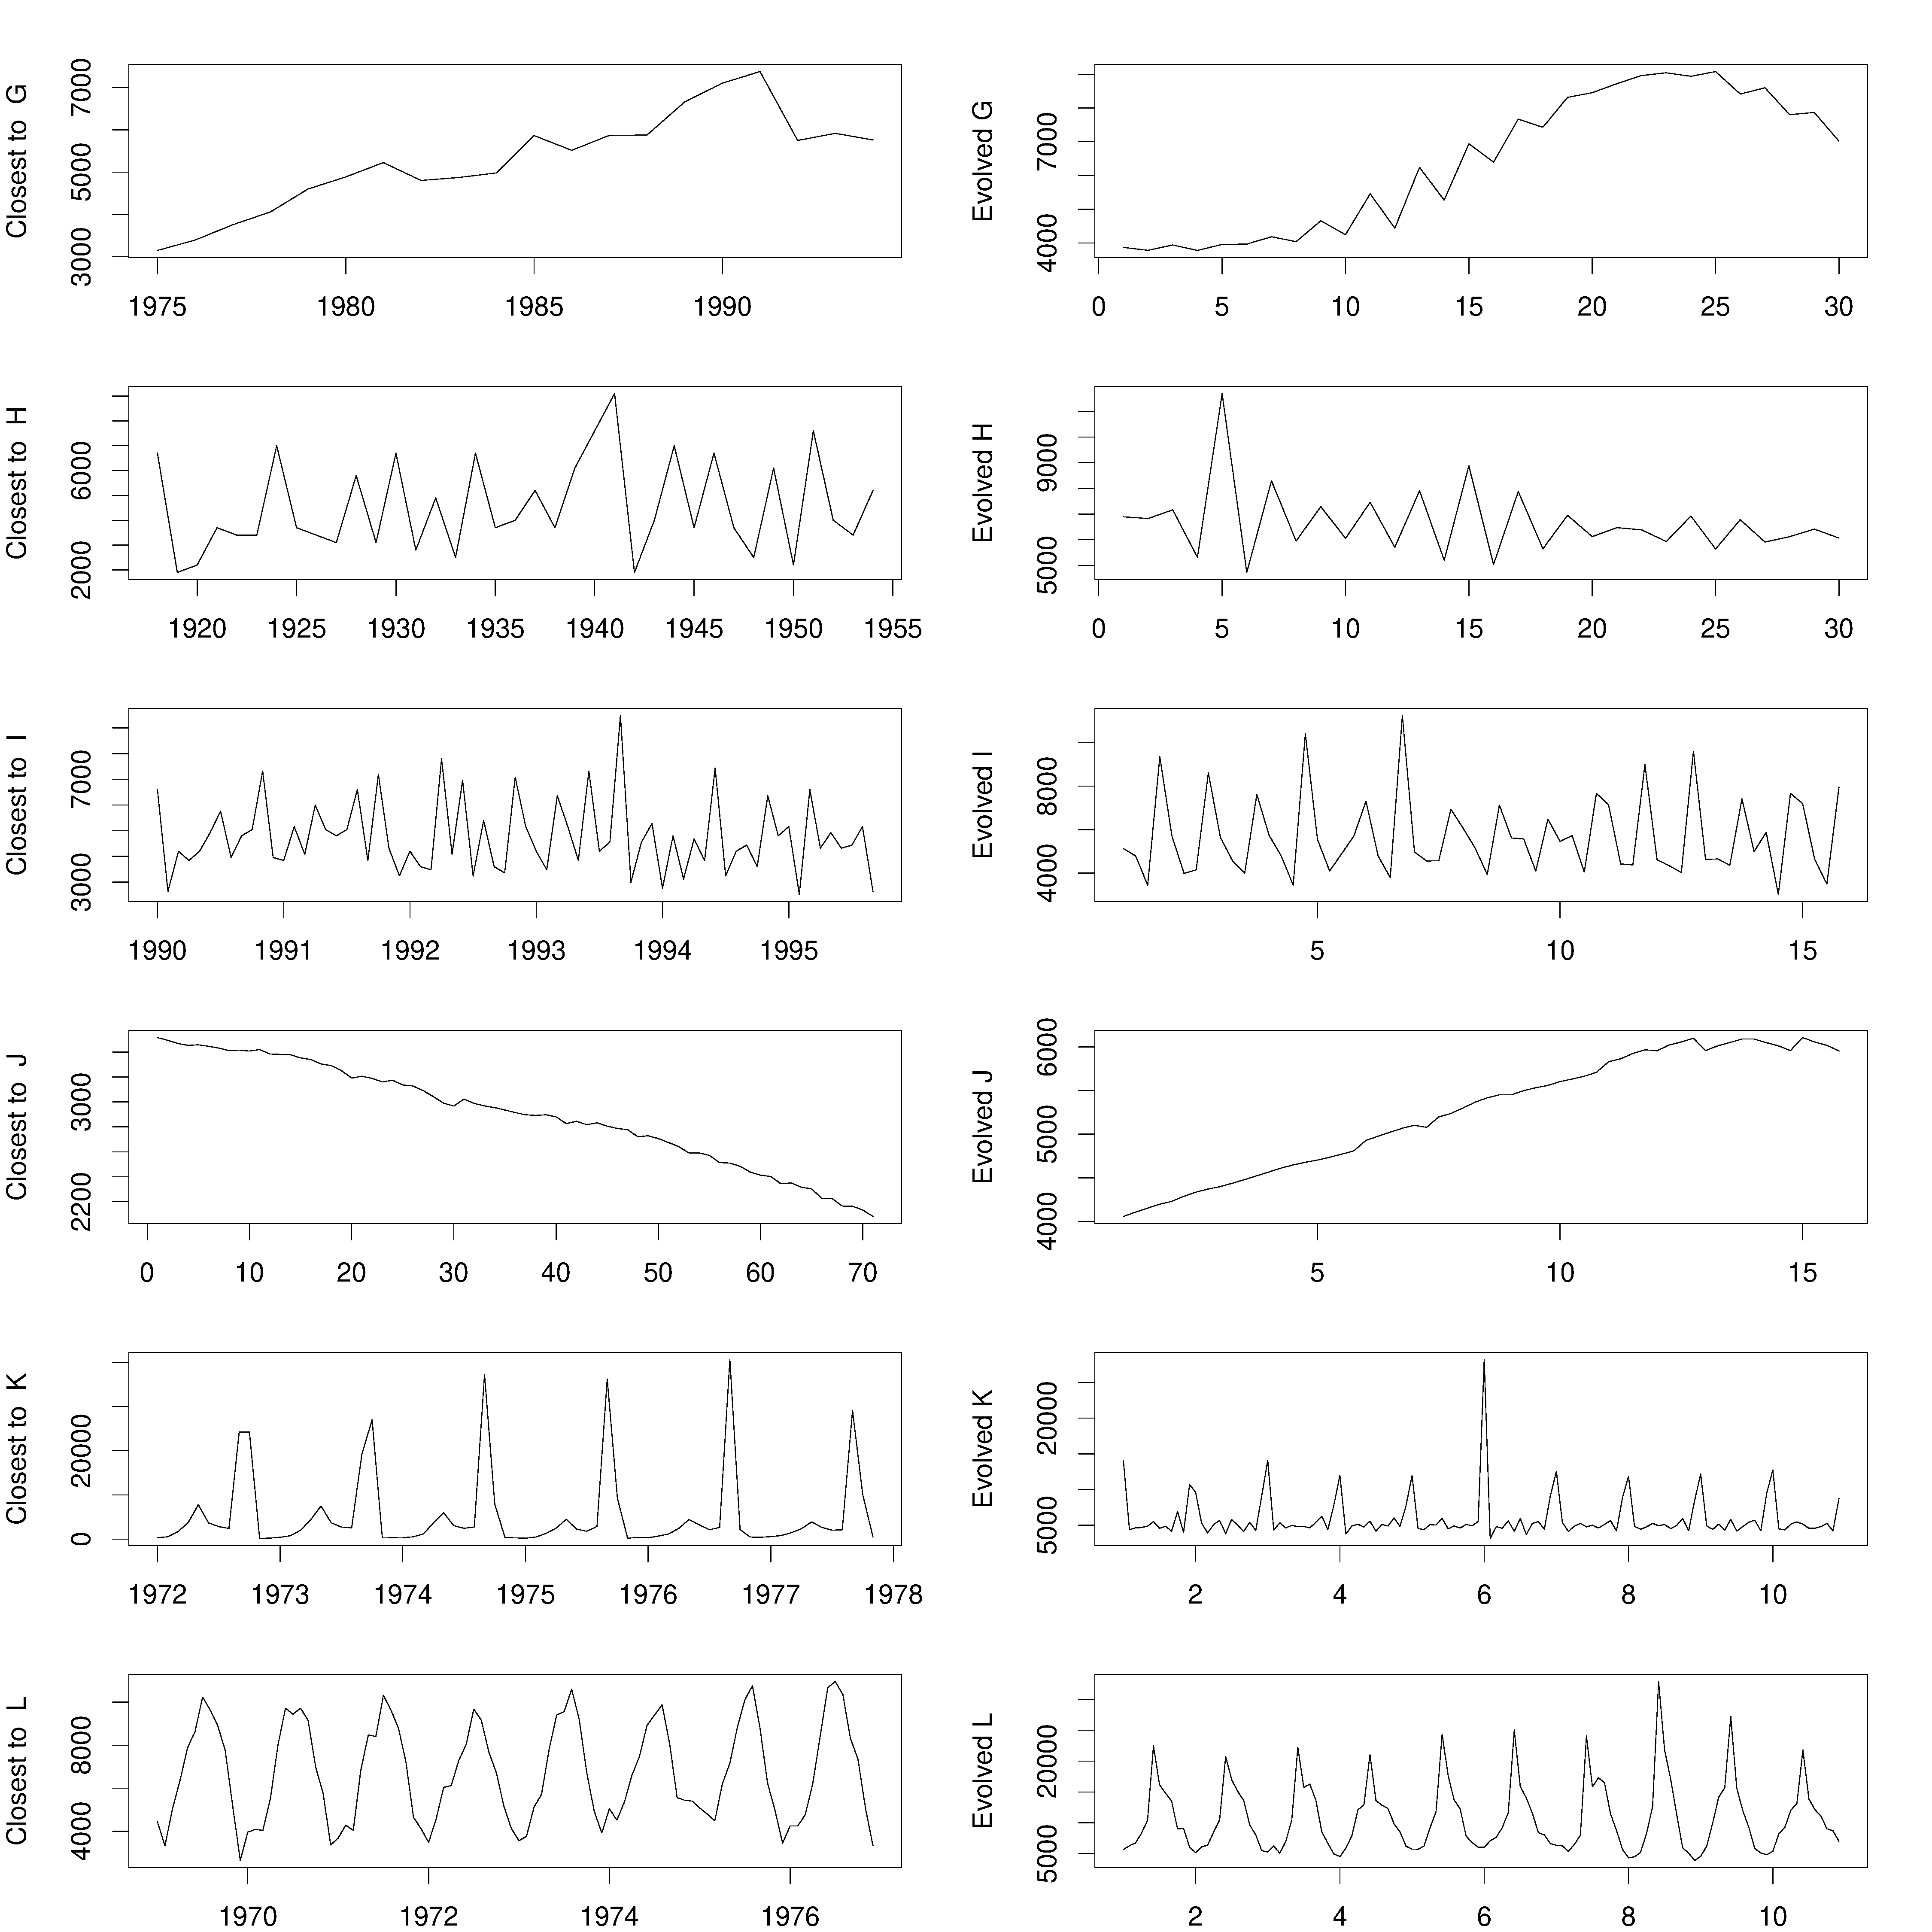
\includegraphics[width=0.7\textwidth]{figures/UnknownEvolvedEgs.pdf}

\end{frame}

\begin{frame}{Target points}

\begin{itemize}
\item
  32 *32 grid with 1024 points, which are bounded within one unit wider
  than the upper and lower bounds of PC1 and PC2.
\item
  Generate 1024 yearly, quarterly and monthly time series that are
  previously unknown and evolved by maximising the fitness function.
\end{itemize}

\end{frame}

\begin{frame}{Results}

\centerline{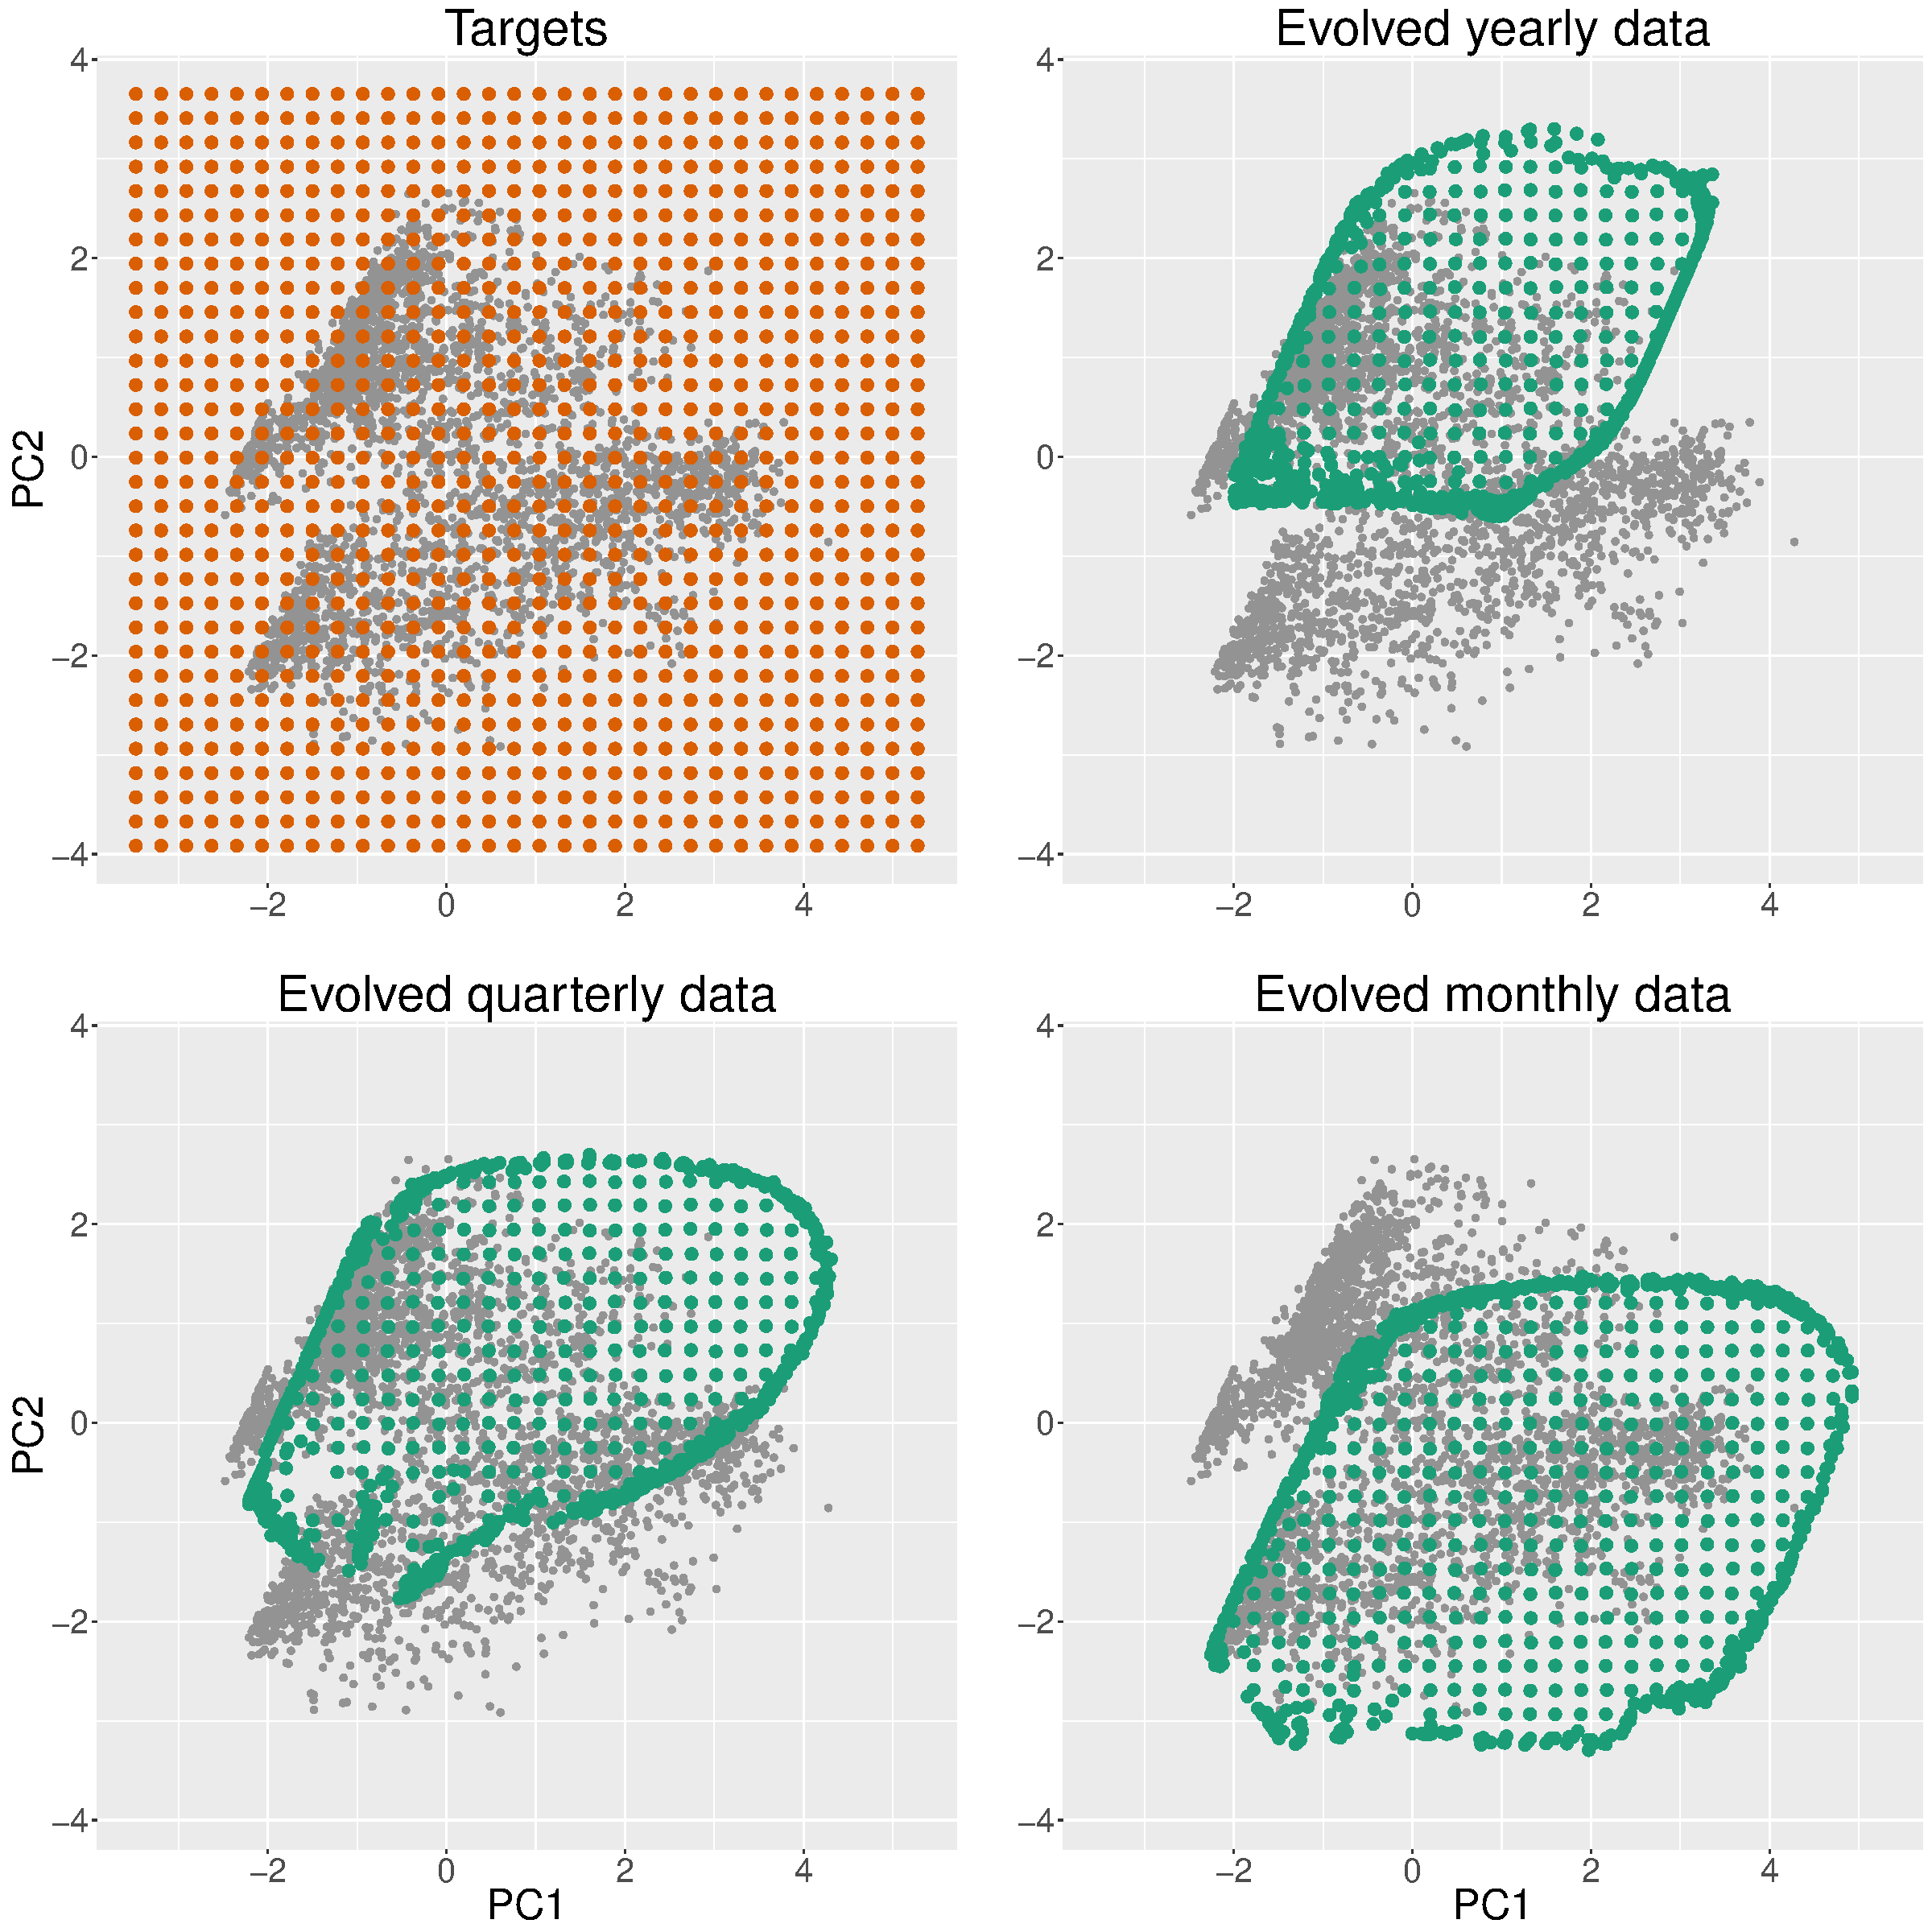
\includegraphics[width=\textwidth]{figures/EvolvedTSnbDiffLsep.pdf}}

\end{frame}

\section{Comparison of time series forecasting methods in the feature
space}\label{comparison-of-time-series-forecasting-methods-in-the-feature-space}

\begin{frame}{No-free-lunch}

\begin{itemize}
\item
  There is never likely to be a single method that fits all situations.
\item
  There is no time series forecasting method that will always perform
  best. Even for one particular time series, no one technique is
  consistently superior to others.
\end{itemize}

\end{frame}

\begin{frame}{Time series forecasting methods}

\begin{enumerate}
\def\labelenumi{\arabic{enumi}.}
\tightlist
\item
  Naïve: using the most recent observation as the forecast.
\item
  Seasonal naïve: forecasts are equal to the most recent observation
  from the corresponding time of year.
\item
  The Theta method, which performed particularly well in the
  M3-Competition.
\item
  ETS: exponential smoothing state space modelling.
\item
  ARIMA: autoregressive integrated moving average models.
\item
  STL-AR: an AR model is fitted to the seasonally adjusted series, while
  the seasonal component is forecast using Seasonal naïve.
\end{enumerate}

\end{frame}

\begin{frame}{Minimum MASE of M3}

\begin{figure}[htbp]
\centering
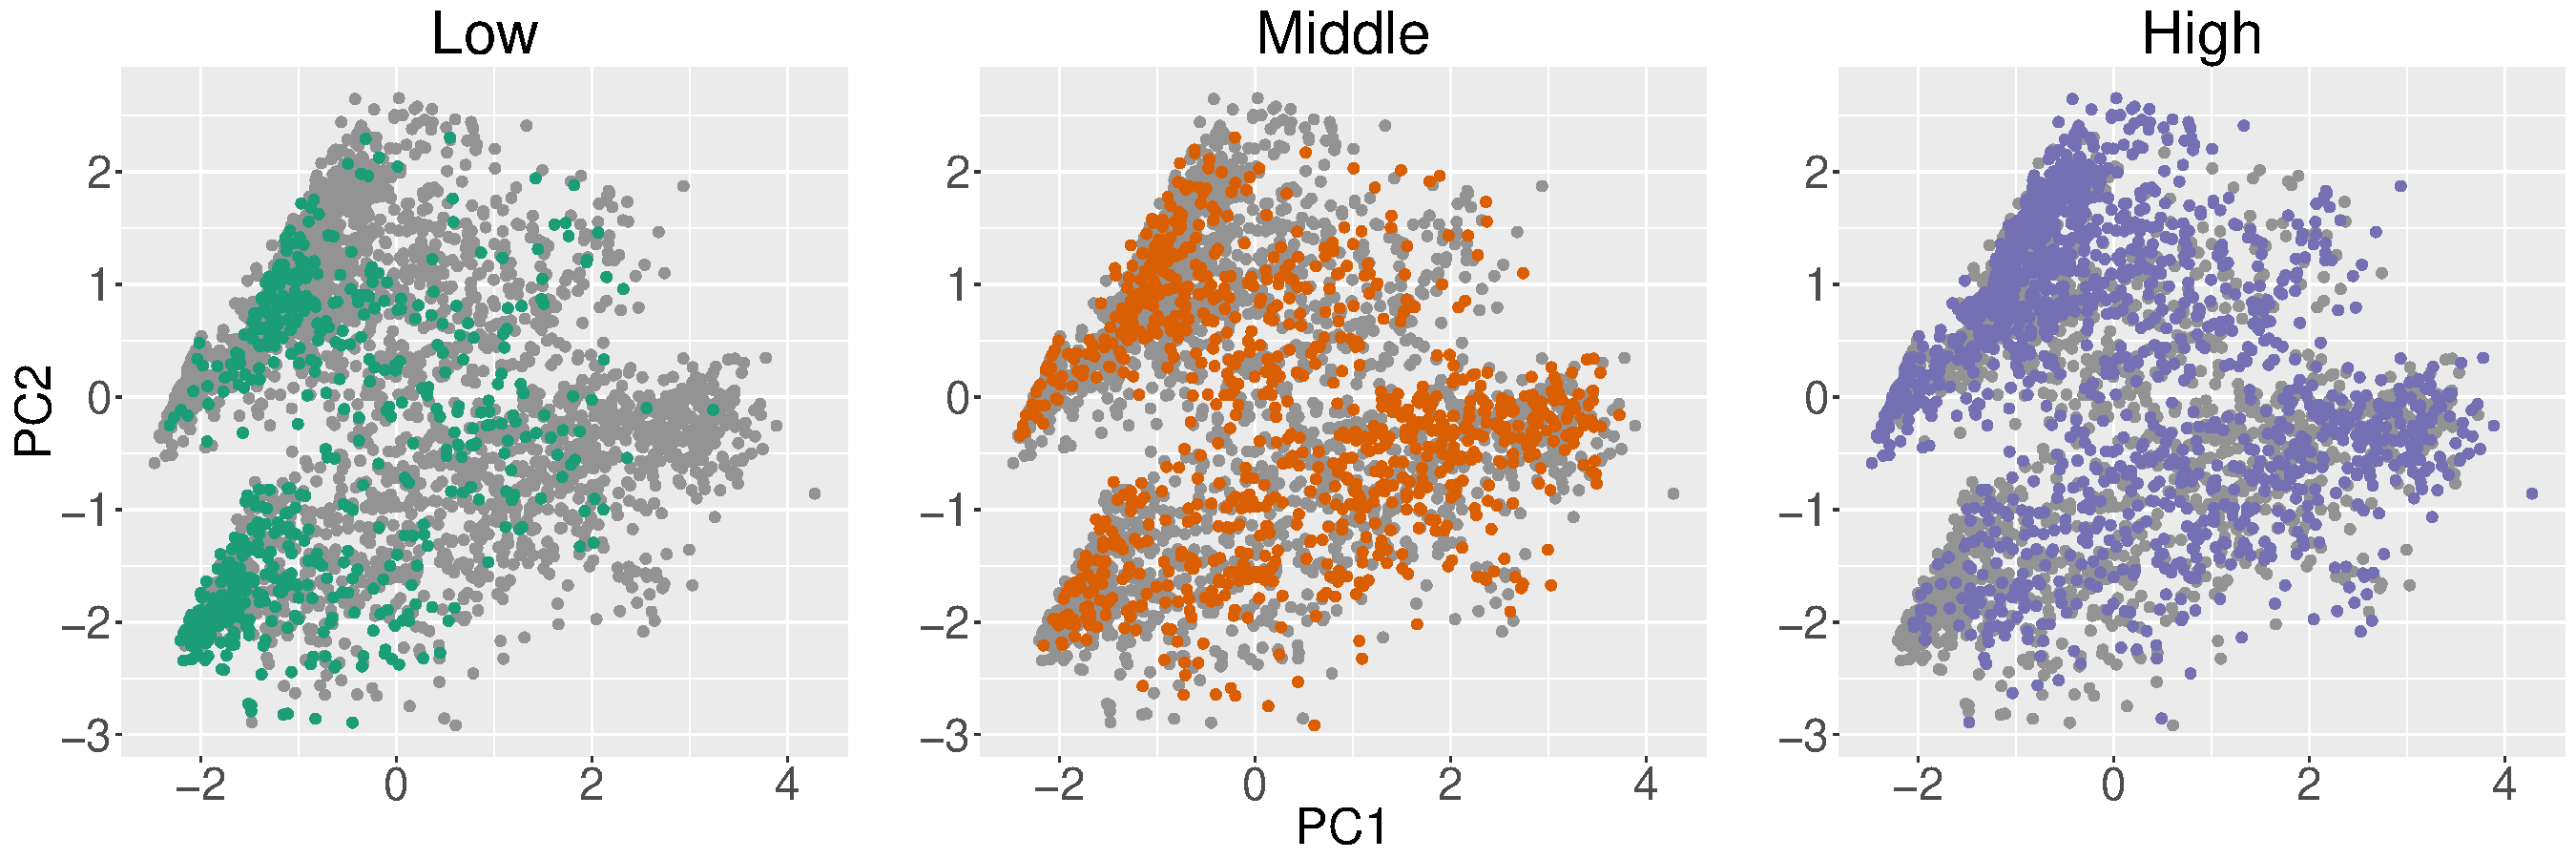
\includegraphics{figures/minMASE.pdf}
\caption{Locations of M3 series which achieve Low, Middle and High
minimum MASE from all the six forecasting algorithms.}
\end{figure}

\end{frame}

\begin{frame}{MASE of M3}

\centerline{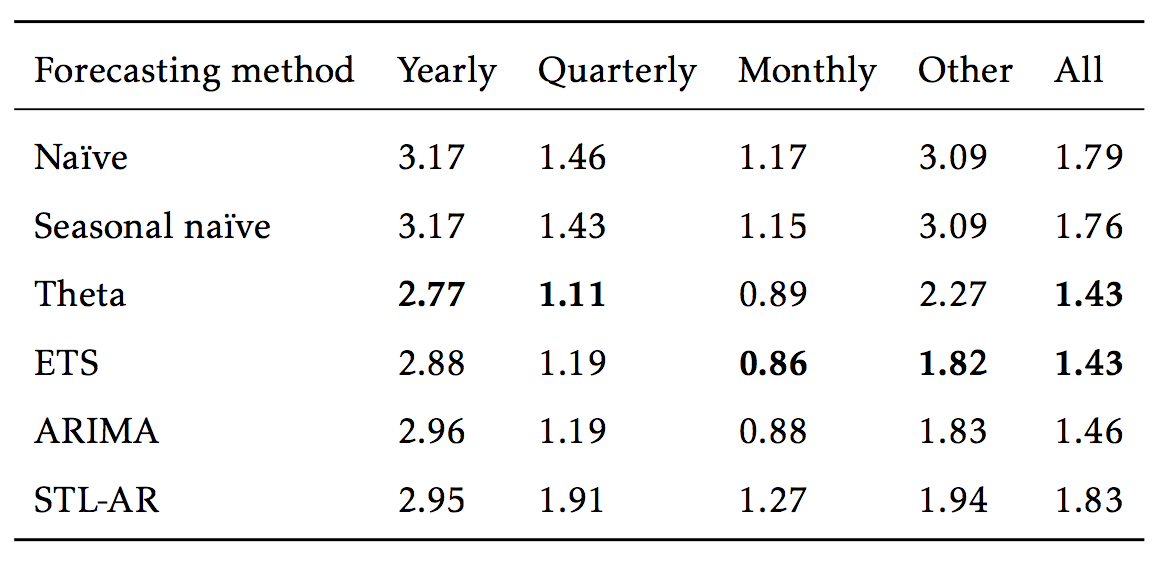
\includegraphics[height=2in]{figures/table1.png}}

\end{frame}

\begin{frame}{MASE of evolved series}

\centerline{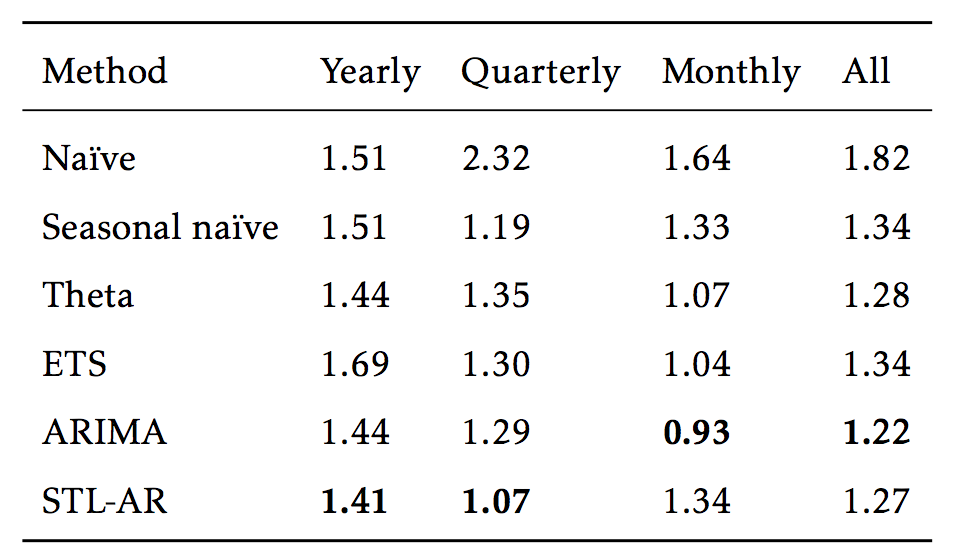
\includegraphics[height=2in]{figures/table2.png}}

M3 is not a representative sample of any larger population of time
series.

\end{frame}

\begin{frame}{Comparison of forecasting methods}

\centerline{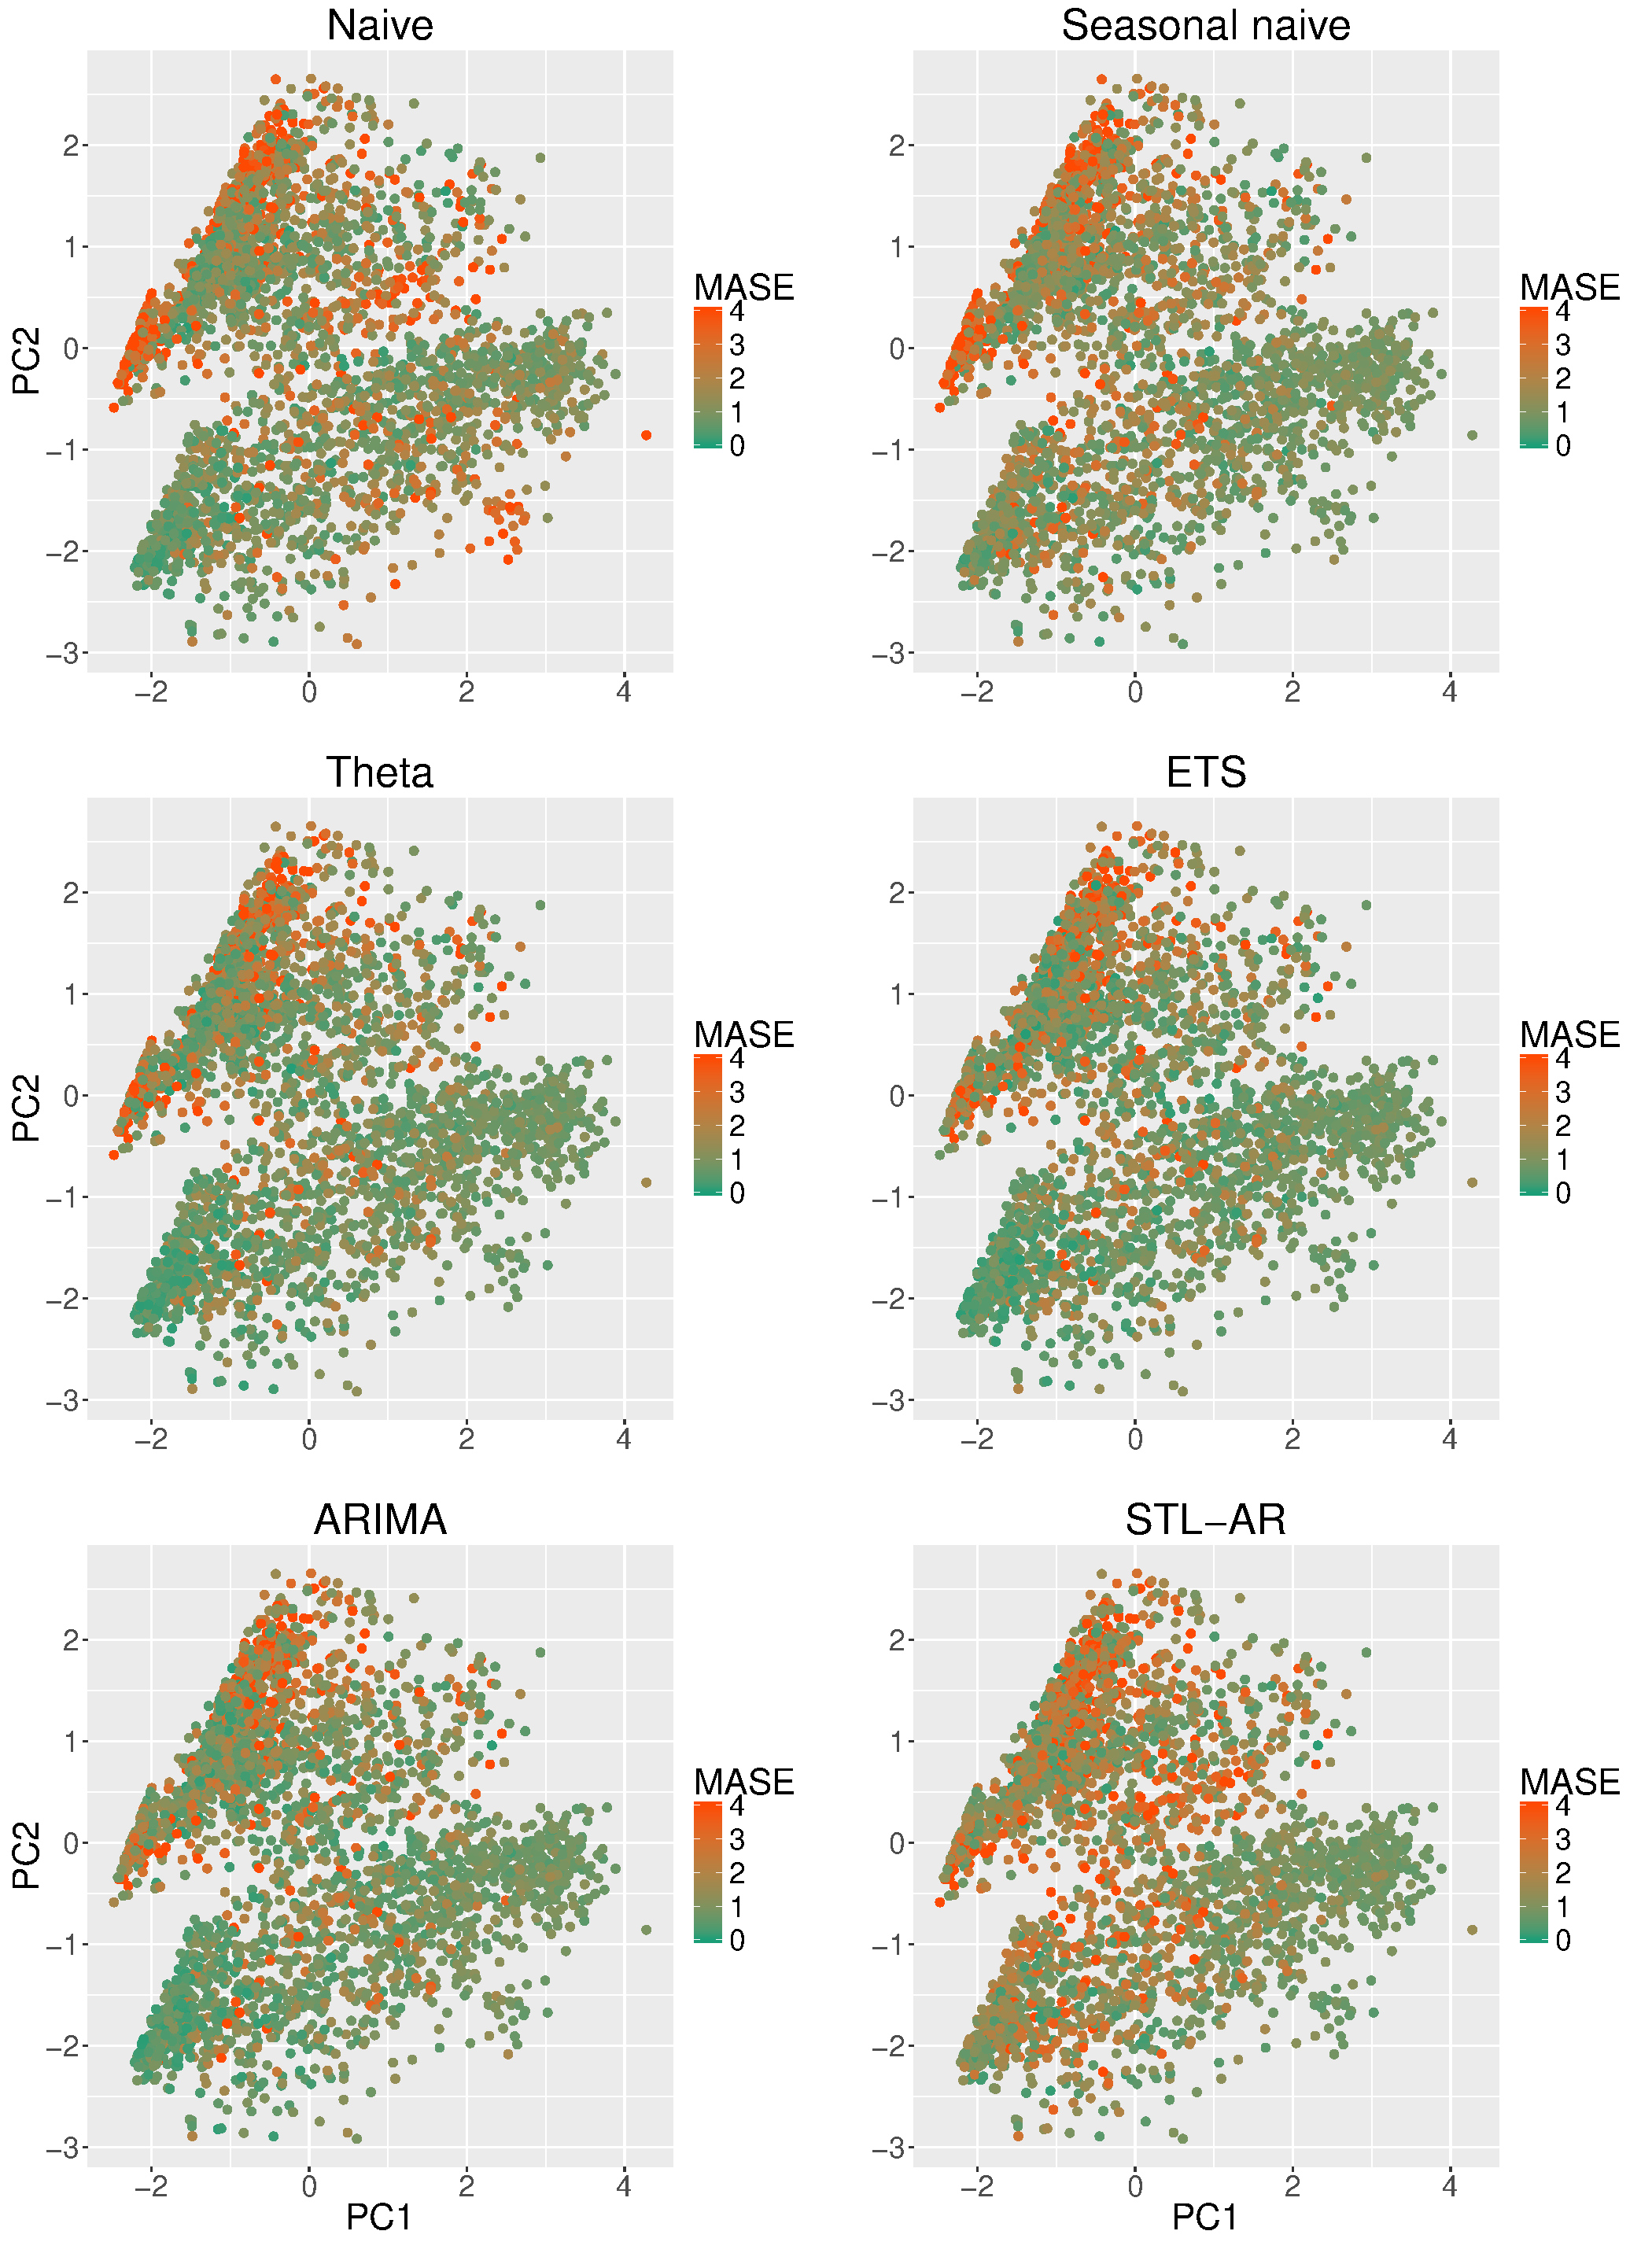
\includegraphics[height=3in]{figures/MASErainbowPlots.pdf}}

\end{frame}

\section{Conclusions}\label{conclusions}

\begin{frame}{Conclusions}

\begin{block}{Identify unusual time series}

\centerline{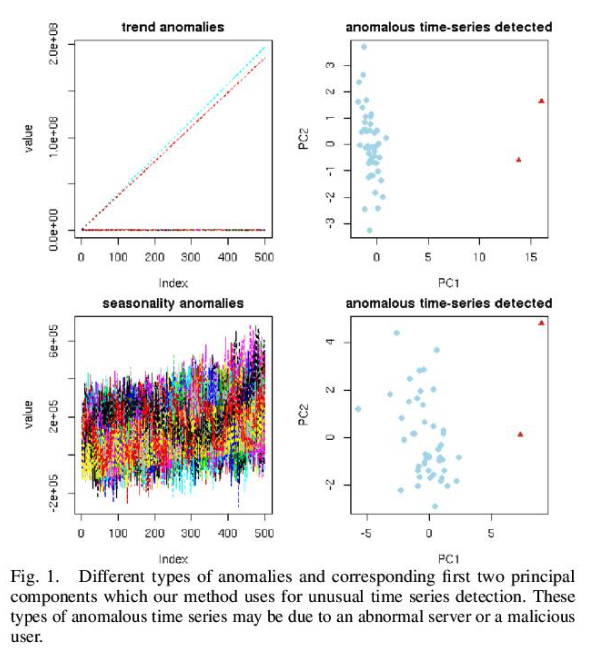
\includegraphics[height=3in]{figures/unusual.png}}

\end{block}

\end{frame}

\begin{frame}{Conclusions}

\begin{block}{Find clusters}

\centerline{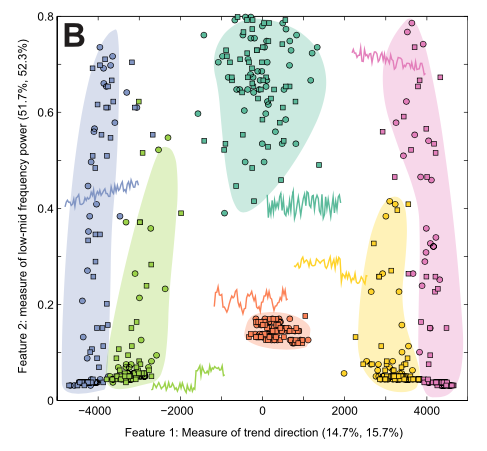
\includegraphics[height=3in]{figures/clustering2.png}}

\end{block}

\end{frame}

\begin{frame}{Conclusions}

\begin{block}{Find clusters}

\centerline{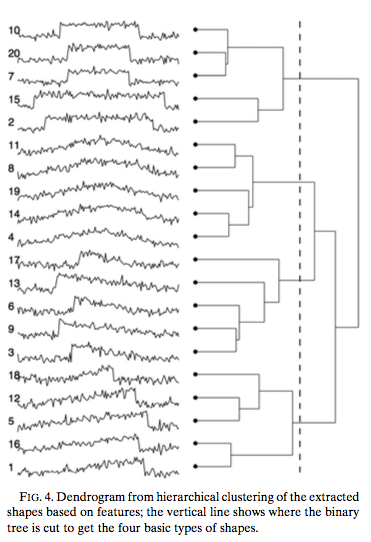
\includegraphics[height=3in]{figures/clustering1.png}}

\end{block}

\end{frame}

\begin{frame}{Conclusions}

\begin{itemize}
\tightlist
\item
  Generate new time series with specific features.
\item
  M3 conclusions will not necessarily hold for other time series
  collections.
\item
  Different forecasting methods perform better in some regions of the
  feature space than other methods.
\end{itemize}

\end{frame}

\begin{frame}{What else can we do}

\begin{itemize}
\tightlist
\item
  Develop meta-forecasting algorithms which choose a specific method
  based on the location of a time series in the instance space (almost
  done).
\item
  Generate new time series with specific features with decent
  computation efficiency (almost done.)
\item
  Develop \textbf{R} package \textbf{TSfeatures} which can extract
  thousands of features from a single time series (\textbf{to be done,
  now}).
\item
  Select features automatically for a variety of tasks (\textbf{to be
  done}).
\item
  Applications (\textbf{to be done}).
\end{itemize}

\end{frame}

\begin{frame}{References}

Yanfei Kang, Rob J. Hyndman, Kate Smith-Miles. Visualising forecasting
algorithm performance using time series instance spaces.
\emph{International Journal of Forecasting} 33 (2), 345-358 (2017).

Ben D. Fulcher, Nick S. Jones. Highly comparative feature-based
time-series classification. \emph{IEEE Transactions on Knowledge and
Data Engineering}, 26(12), 3026-3037 (2014). Code available at
\url{https://github.com/benfulcher/hctsa}.

\Large \url{http://yanfei.site}

\Large \href{mailto:yanfeikang@buaa.edu.cn}{\nolinkurl{yanfeikang@buaa.edu.cn}}

\end{frame}

\end{document}
